\begin{frame}{DNN Reco}
    \begin{itemize}
        \item \texttt{dnn\_reco} \footnote{\href{https://github.com/icecube/dnn_reco/}{github.com/icecube/dnn\_reco/}}
              software by Mirco Hünnefeld (in \texttt{python3} based on \texttt{Tensorflow})
        \item Versatile network design using hexagonal convolutional layers
        \item Training data generation and normalization for IceCube
        \item Weighted adaptive multi-label training
        \item DNN Based reconstruction methods already outperformed classical ones in:
              \begin{itemize}
                  \item cascade energy
                  \item cascade direction
                  \item muon track energy
                        \item[\color{mLightBrown}$\Rightarrow$]<2-> {\color{mLightBrown} muon track direction?}
              \end{itemize}
    \end{itemize}
\end{frame}
\begin{frame}{DNN Reco Feature Generation}
    \begin{figure}
        \centering
        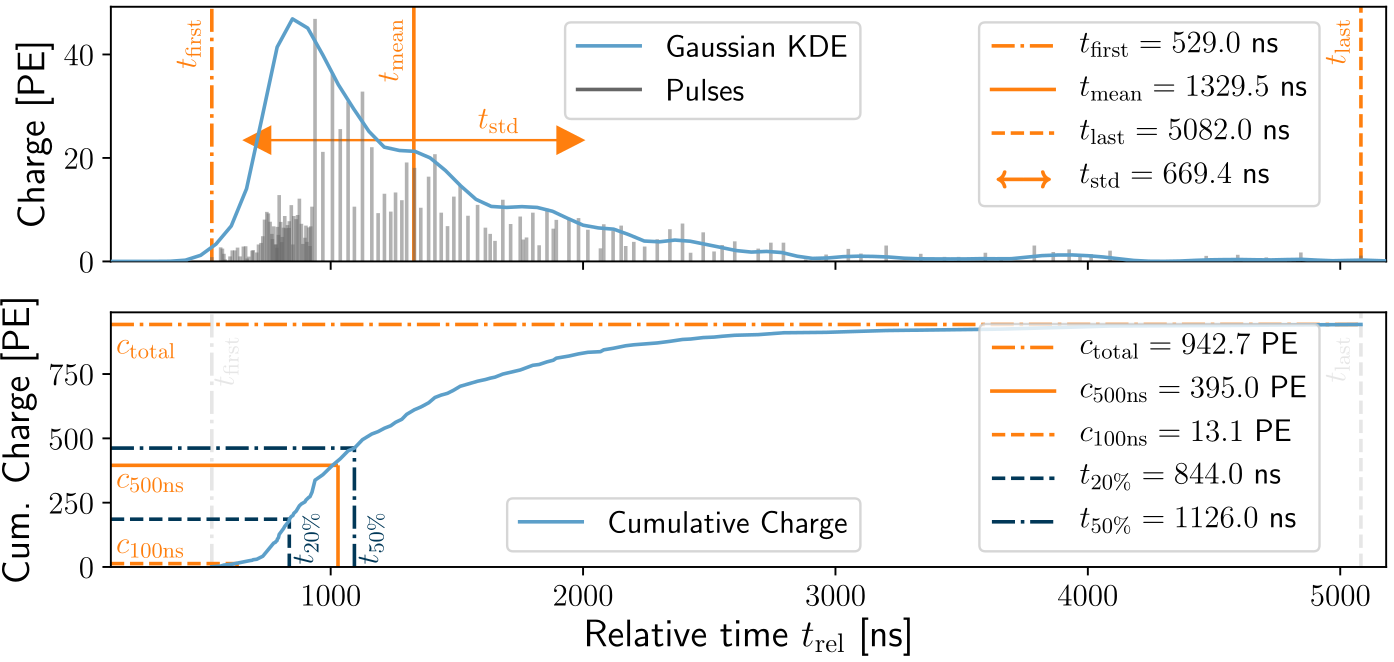
\includegraphics[width=.8\textwidth]{media/feature_generation}
        \caption*{Feature generation [\fullcite{DNNReco}]}
    \end{figure}
\end{frame}
\begin{frame}{Neural Network Layout}
    \begin{columns}
        \begin{column}{.6\textwidth}
            \begin{figure}
                \centering
                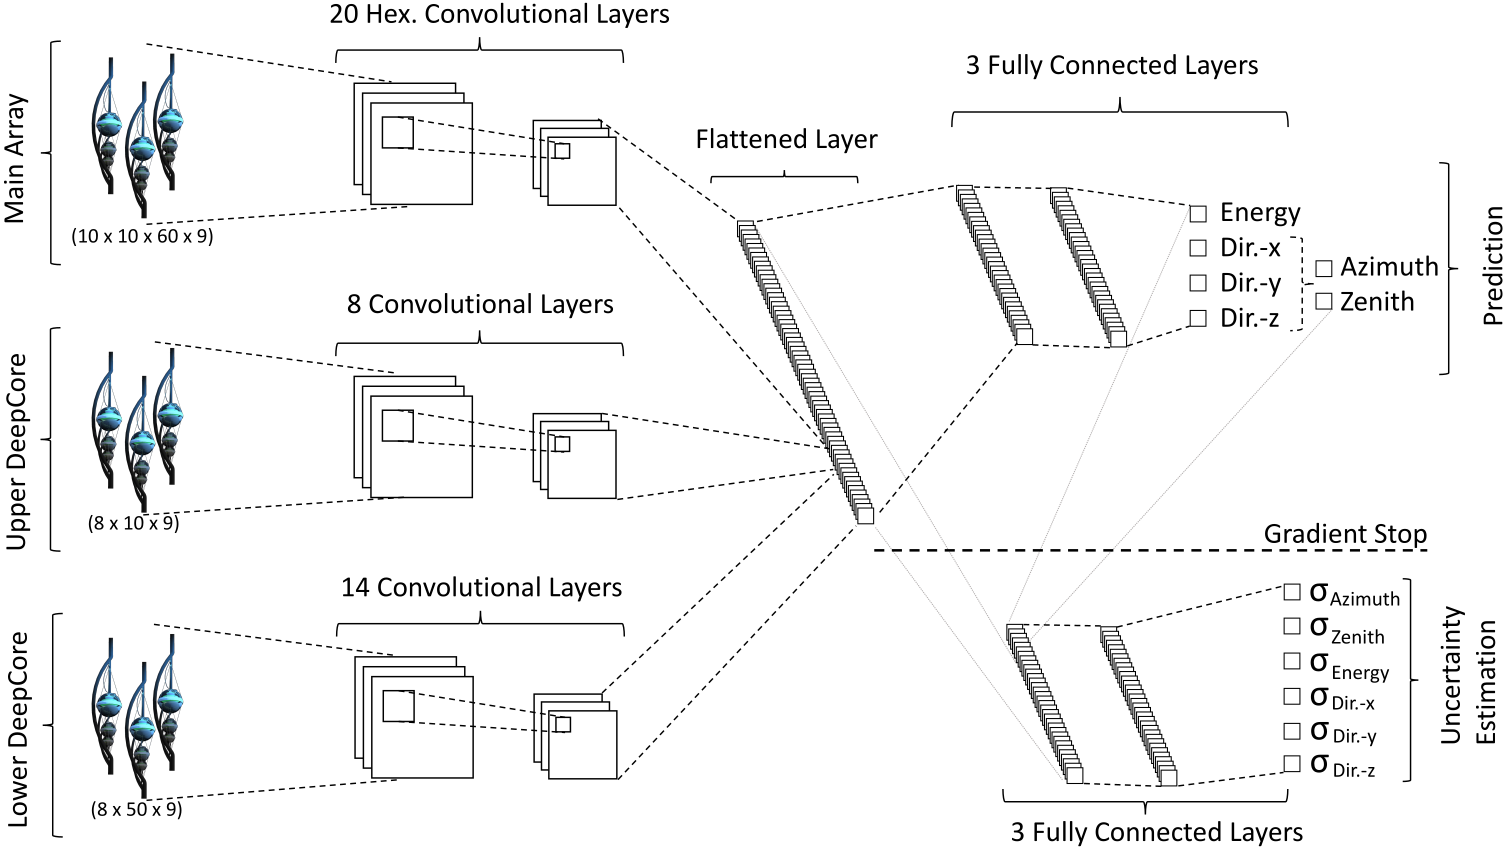
\includegraphics[width=\textwidth]{media/network_design.png}
                \caption*{Network Layout \footnotemark[1]}
            \end{figure}
            \vspace{-1em}
            $\hat f(\mathbf{X}_i|\vec p)$ = NN
            and $\vec p$ = trainable parameters
        \end{column}
        \begin{column}{.4\textwidth}
            \onslide<2->{
                Adjustable hyperparameters:
                \begin{itemize}
                    \small
                    \item Size and number of (hexagonal) convolutional layers
                    \item Size and number of dense layers (in uncertainty subnetwork)
                    \item Batch size
                    \item Input features
                    \item Loss function
                    \item Dropout rate
                    \item Activation function
                    \item Many more!
                \end{itemize}
            }
        \end{column}
    \end{columns}
    \vspace{1em}
    \footnotetext[1]{Taken from \fullcite{DNNReco}}
\end{frame}
\begin{frame}{Hexagonal Convolutional Layers}
    Used to exploit rotational/translational symmetries
    \begin{figure}[htbp]
        \centering
        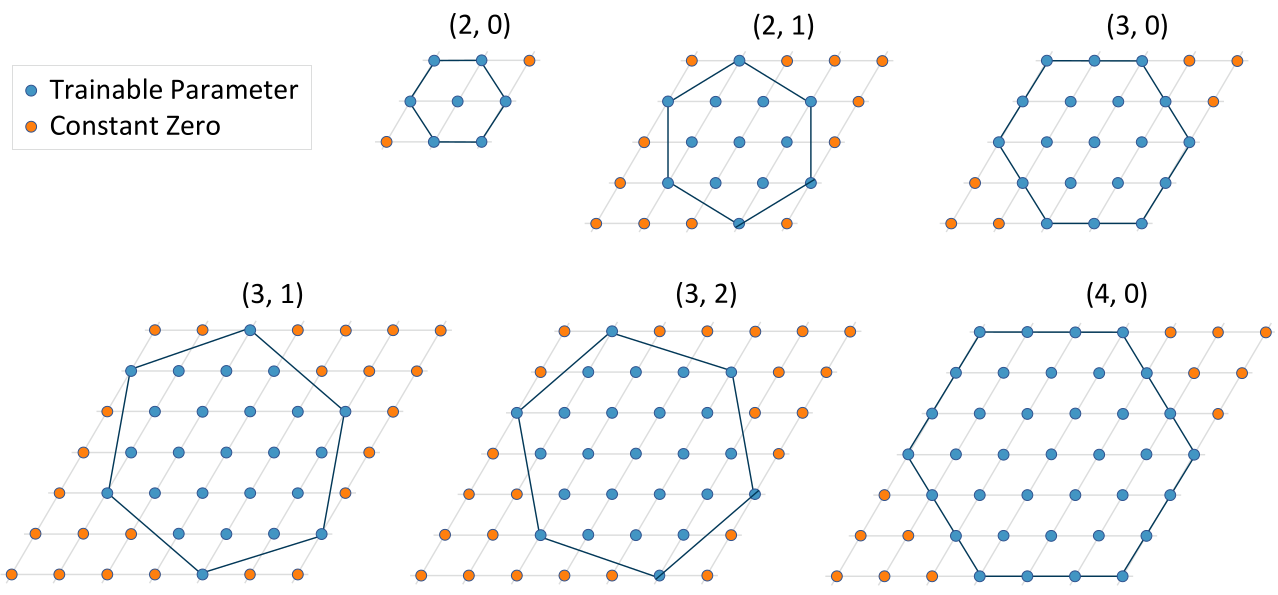
\includegraphics[width=.7\textwidth]{media/hexagonal_layers.png}
        \caption*{Implementation of hexagonal convolutional kernel \footnotemark[1]}
    \end{figure}

    \footnotetext[1]{Taken from \fullcite{DNNReco}}
\end{frame}
\begin{frame}{Loss Function and Uncertainty Estimation}
    Let's look at the single event, single feature  loss function.\\
    Example: $y=\theta$ and $\sigma_y$ is the uncertainty estimate. \\
    Prime means \emph{normalized} and weighted (for multi-feature regression)\\
    \vspace{1em}
    Mean Square Error:
    \begin{equation*}
        L(y_{\mathrm{pred}}, \sigma_y|y_{\mathrm{true}}) =
        \underbrace{\l(y'_{\mathrm{pred}} - y'_{\mathrm{true}}\r)^2}_{L_{\mathrm{pred}}}
        +
        \underbrace{\l(\sigma'_{y} - {\mathtt{\tiny gradient\_stop}}\l(\abs{y'_{\mathrm{true}} - y'_{\mathrm{true}}}\r)\r)^2}_{L_{\mathrm{unc}}}
    \end{equation*}
    \pause
    Gaussian Likelihood (more sensitive):
    \begin{equation*}
        L(y_{\mathrm{pred}}, \sigma_y|y_{\mathrm{true}}) =
        2\ln{\sigma'_y}+\l(\frac{y'_{\mathrm{true}}-y'_{\mathrm{pred}}}{\sigma'_y}\r)^2
    \end{equation*}
\end{frame}